\documentclass[letterpaper,12pt]{report}
\usepackage[english]{babel}							%For internationalization
\usepackage[utf8]{inputenc}							%For character encoding
\usepackage{amsmath}								%For mathematical typesetting
\usepackage{amssymb}								%For mathematical typesetting
\usepackage{graphicx}								%For handling graphics
\usepackage[top=1in, bottom=1in, left=1.5in, right=1in]{geometry}	%Sets required thesis margins
\usepackage[nodisplayskipstretch,doublespacing]{setspace} 		%Sets required thesis double spacing
\usepackage{titlesec} 								%Used to easily redefine section title styles
\usepackage{listings}								%Code formatting

\newcommand{\be}{\begin{equation}}
\newcommand{\ben}[1]{\begin{equation}\label{#1}}
\newcommand{\ee}{\end{equation}}
\newcommand{\aomega}{\overset{\sim}{\omega}}				%Approximate omega

\title{Vortex Dominated Flows: A High-Order, Conservative Eulerian Simulation Method}
\author{Josh Bevan}
\date{\today}

%Set section formats so chapters, sections, and subsections are 14ish pt
\titleformat{\section}{\large\bfseries}{\thesection}{1em}{}
\titleformat{\subsection}{\normalsize\bfseries}{\thesubsection}{1em}{}
\titleformat{\chapter}{\large\bfseries}{\thechapter}{1em}{}
	\titlespacing*{\chapter}{0pt}{.7in}{0pt} %Add whitespace above chapter title to get a 2in margin

%Frontmatter----------------------------------------------------------------------
\begin{document}
\pagenumbering{roman} %Roman numbering for frontmatter
\maketitle
\begin{abstract}
\setcounter{page}{2} %Manual page numbering because 'abstract' is annoying
\thispagestyle{plain} %Needed to show page number as pagestyle was reset to 'empty' when \maketitle is called internally
A high-order, conservative Eulerian method will be presented for the simulation of vortex dominated inviscid fluid flows. The primitive variable incompressible Euler equations are recast in the velocity-vorticity form to explicitly enforce conservation of vorticity. The advection of the vorticity is then calculated via a two-step process: the velocity field is first determined by evaluation of the Biot-Savart integral, and then a line-based discontinuous Galerkin (DG) Eulerian spatial discretization scheme is applied to accurately advect the vorticity field. The accuracy and convergence of this method is examined for test cases where an analytical solution exists, as well as more challenging test cases which lack an analytical solution. The influence the velocity field discretization has on the performance of the method is of particular interest.
\end{abstract}

\setcounter{page}{3} %Manual page numbering because 'abstract' is annoying
\chapter*{Acknowledgments}
\begin{singlespace} %Tables should be single spaced
\tableofcontents
\listoftables
\addcontentsline{toc}{section}{List of Tables}
\listoffigures
\addcontentsline{toc}{section}{List of Figures}
\end{singlespace}

%Here we change the pagestyle so that the page number appears top right. We need to redefine the \chapter command to change the default pagestyle from 'plain' to 'myheadings'
\pagestyle{myheadings}
\makeatletter
\renewcommand\chapter{\if@openright\cleardoublepage\else\clearpage\fi
                    \thispagestyle{myheadings}% original style: plain
                    \global\@topnum\z@
                    \@afterindentfalse
                    \secdef\@chapter\@schapter}
\makeatother

%Mainmatter-----------------------------------------------------------------------
\chapter{Introduction}
\pagenumbering{arabic} %Reset to arabic numbering for mainmatter
\section{Velocity-Vorticity equation}
Direct solution of Navier-Stokes is impractical for many fluid problems and where possible simplifications should be made; one such possibility is for vortex dominated flows. It is possible to recast Navier-Stokes from a primitive variable form ($u,v,p$) to a velocity-vorticity ($u,v,\omega$) form. This has several advantages: explicit conservation of vorticity, elimination of pressure, and reduction of required simulated degrees of freedom to just those that form the vorticity support. For inviscid and incompressible flows the vorticity transport equation is:
\ben{VV3D} \frac{\partial \omega}{\partial t} + u \cdot \nabla \omega - \omega \cdot \nabla u = S(x,t)\ee

Traditionally simulation techniques take advantage of Helmholtz and Kelvin's theorems; vorticity exists as material surfaces, lines, etc. and therefore a Lagrangian approach is natural. Typically the vorticity is discretized into vortex particles, lines, or sheets at which point advection becomes trivial, one merely needs to calculate the velocity field at each particle and step forward in time \cite{Strain1996,MoussaCarley2008,KoumLeonard1995}. Several monographs exist that enumerate the details and advantages of Lagrangian vortex methods \cite{Lugt1983,Saffman1992,Speziale1987}.

\section{Lagrangian Methods}
There are several variations of Lagrangian methods depending on how the vorticity is discretized; point vortex methods were the earliest with the work of Rosenhead \cite{Point1} in 2D with singular point vortices, which was later built upon and improved \cite{Point2,Point3,Point4,Point5,Point6}. Higher dimensional discretizations take the form of vortex line \cite{Line1,Line2,Line3,Line4}, sheets \cite{Sheet1,Sheet2,Sheet3}, and volumes \cite{Volumes1,Volumes2,Volumes3}.

The velocity field due to the vorticity is usually calculated from solving the Poisson problem, or through inversion of the Poisson problem via evaluation of the Biot-Savart integral. There are several challenges with evaluation of the velocity: boundary conditions in the Poisson solution method, and singularities in the Biot-Savart volume integral method. Typically Lagrangian point vortex codes de-singularize the kernel \cite{Rosenhead1930,Moore1972}. Direct summation for the velocity field has a $\mathcal{O}(N^2)$ complexity. Tree-codes \cite{LindsayKrasny2001} and Fast Multipole Methods (FMM) \cite{Strain1997} are common ways of achieving a more efficient.

The convergence of vortex methods was proven early on in 2D \cite{Convg2D} and was later extended to 3D \cite{Convg3D}.

\section{Lagrangian Method Difficulties}
Lagrangian point methods present several problems. Point disorganization can occur as the fluid evolves, this typically requires temporary meshing to recondition the discretization. This has been handled with various methods; recalculation of the quadrature weights at each time step \cite{Remesh2,Remesh3}, regridding/rezoning \cite{Remesh4}, and remeshing \cite{Remesh5} among them. Additionally, most Lagrangian approaches are limited to low order; careful point locations must be chosen and maintained through frequent remeshing etc. in order to achieve high-order convergence \cite{Strain1997}.

\section{Existing Eulerian codes}
In comparison, far less literature exists for Eulerian approaches. Chief among them is the work of Brown et al. \cite{Brown2000} who adapted the velocity-vorticity approach to a low order Finite Volume (FV) solver. Later they were able to extend their method to be accelerated via a FMM \cite{Brown2004}. However, like most FV approaches, to extend to high order solution approximations requires extended stencils that ultimately limit the geometrical freedom of the mesh. Steinhoff et al. also used an Eulerian approach, but solved a modified form of the inviscid Euler equations with "vorticity confinement" rather than the velocity-vorticity equation \cite{SteinhoffUnderhill1994}.
%
\section{Proposed Method}
\subsection{Alternate Advective Methods}
The desire to resolve fine vortical structures motivates the need for a high order solver. Considering the challenges associated with achieving a high order Lagrangian method and the preliminary success of Brown et al.'s low order method, it is natural to attempt a high order Eulerian vorticity-velocity method, but what of the spatial discretization choice?

Finite difference methods suffer from similar problems as FV with extended stencils, as well as not being explicitly conservative. A finite element approach is ill-suited to the hyperbolic nature of vorticity advection. Spectral methods are promising, but for sparse vorticity domains are less-efficient due to the global support of the harmonic bases. However, discontinuous Galerkin (DG) methods are a natural choice; they are conservative, able to take advantage of vorticity sparseness, are well-suited to handle advection via intelligent choice of a numerical flux function, and have bases with local/compact support.

For domains free of impinging bodies a hexahedral mesh with a tensor product grid of interpolation points is convenient to implement. This permits the use of a line-DG \cite{Persson2013} approach that considerably simplifies multi-dimensional cases by allowing reuse of 1D methods. A 2D domain will be considered to evaluate whether the method is practical, as well as to limit solution times to those that are reasonable on a workstation. This has the advantage of removing the vortex stretching term and reducing the vorticity to a scalar. The resultant partial differential equation (PDE) takes on the familiar form of a scalar conservation law.

\subsection{Velocity Field Fidelity}
Unlike Lagrangian methods where advection is trivial, or Brown's method which is at low order, the necessary fidelity of the velocity field to maintain a particular global convergence rate that one would expect from the order of the vorticity field is not immediately obvious. The method by which one recovers the velocity field is decoupled from the advective solver, which has no a priori knowledge or assumptions about the quality of the velocity field approximation. 

To maintain maximum flexibility for investigative purposes and to remove as much approximation error as possible the velocity field for validation of the underlying method is calculated via direct evaluation of the BS integral.

\section{Thesis Goals and Structure}
The overarching thesis goal is the development of a high-order solver capable of modeling inviscid incompressible vorticity-dominated flows in 2D. In order to accomplish this several ancillary goals must be achieved: construction of a high-order advective solver capable of mixed order flux handling, and a high-order Biot-Savart evaluation routine that is as efficient as can be achieved within the bounds of a direct summation approach.

At it's conclusion the chief contributions will be: a complete solver routine that integrates all necessary subsystems, validation of the solver and the underlying Eulerian vortex approach; and evaluation of the convergence, error, and performance of the method and solver.

In Chapter 2, a brief overview of the underlying theory of the velocity-vorticity formulation, velocity evaluation, the Biot-Savart  kernel and the discontinuous Galerkin method are covered. The extension of one-dimensional DG methods to 2D via a line-DG style method will also be reviewed. 

In Chapter 3 the methodology taken to construct a high-order Eulerian velocity-vorticity is covered. Chief among the concerns are the spatial basis, choice of interpolation, and numerical integration of the interpolation.

Chapter 4 covers solver specific implementation details. An introductory overview of the solver structure is first laid out. Then, formation of the semi-discrete system, along with the development of some specialized tools are addressed. A high-order velocity evaluation method is laid out, as well as some computation-saving modifications. Explicit time-stepping via a Runge-Kutta method optimized for the spectra of the DG operator is briefly reviewed.

In Chapter 5  a test plan is laid out for validation and investigation of the overall solver and method. Results of the validation tests, convergence studies, and performance of the possible improvements and modifications is presented. Additionally runtime performance of the solver is examined, dependent on solver parameters, tolerances, order, etc.

In Chapter 6 the successful performance of the method and solver is presented and discussed. Additionally an un-implemented extension to the velocity evaluation via a modified Fast Multipole Method is presented. Chapter 7 points in the direction of possible expansion of the method to include additional physical behaviors and configurations, as well as several next steps that should be taken to improve the solver for practical solution of larger problems beyond what is currently possible.

Finally, Chapter 9 presents the specific implementation details necessary to implement the solver practically and efficiently. Several Matlab functions and routines are presented that either makeup the solver itself, or necessary auxiliary tools that are tangentially needed.
%------------------------------------
\chapter{Theory}
\section{Navier-Stokes: Velocity-vorticity form}
The Navier-Stokes momentum equation is
 \be \rho \left(\frac{\partial \mathbf{u}}{\partial t} + \mathbf{u} \cdot \nabla \mathbf{u} \right) = -\nabla \bar{p} + \mu \nabla^2 \mathbf u + \tfrac13 \, \mu \nabla (\nabla\cdot\mathbf{u}) + \rho \mathbf{g}  \ee
where $u$ is the velocity field, $p$ is the pressure field, and $\rho$ is the density. If we restrict ourselves to incompressible flows and define the quantity \textit{vorticity} as
\be \omega = \nabla \times u \ee
Then the traditional form of the Navier-Stokes equations can be recast
\ben{VV3D} \frac{\partial \omega}{\partial t} + u \cdot \nabla \omega - \omega \cdot \nabla u = S(x,t)\ee
where we collect viscous generation of vorticity in $S$.

There are several benefits to the recast form; first, it explicitly conserves vorticity. The vorticity is recoverable from the primitive variable Navier-Stokes, but the diffusive nature of most upwinded advection means coherent vortical structures are quickly smeared. Also, frequently the distribution of the vorticity is quite sparse. The primitive variable form requires the velocity and pressure be evaluated over the whole domain.

In comparison, the velocity-vorticity form only requires velocity to be evaluated in areas of non-zero vorticity. In areas where there is no vorticity, nothing needs to be advected. The sparser and more concentrated the vorticity, the larger the gap in performance between the two forms; this is especially true in 3D domains where the scaling from surfaces to volumes gives even greater opportunity for empty local regions in the domain. 

Additionally, the primitive-variable form requires the pressure be  solved via a separate elliptic equation. The velocity-vorticity form is absent the pressure and automatically ensures satisfaction of continuity.

For 2-D distributions of vorticity, several simplifications can be made. The originally vectorial vorticity becomes a scalar quantity, all vorticity is directed normal to the plane. As a result, the vortex stretching term in \eqref{VV3D} becomes zero. The only non-zero component of $\omega$ is in the z-direction, however the gradient of the velocity field is zero in the z-direction, so the product is therefore zero. The result is
\ben{VV2D} \frac{\partial \omega}{\partial t} + u \cdot \nabla \omega = S(x,t)\ee
or if instead the second term is expressed in terms of the flux of the vorticity (where $f_i(\omega)=u_i\,\omega$):
\ben{VV2DB} \frac{\partial \omega}{\partial t} + \frac{\partial f}{\partial x_i}= S(x,t)\ee

\section{Velocity Field Evaluation: The Biot-Savart Integral}
Since $\omega$ is the quantity of interest in the flowfield solution, the question must be posed: how does one determine the velocity field? For an incompressible flow we can relate the velocity and vorticity by
\be \nabla^2 u = -\nabla \times \omega \ee
If inverted, the Biot-Savart integral is obtained
\ben{BS} u(x^*) = \int_\Omega K(x^*,x) \times \omega(x) dx \ee
where $x^*$ is the point we wish to evaluate the velocity, $x$ is the coordinate in regions of non-zero vorticity, and $K(x^*,x)$ is the singular Biot-Savart kernel
\ben{BSkern} K(x^*,x) = \frac{-1}{4 \pi} \frac{x^*-x}{|x^*-x|^3} \ee

There are several important points to note that are a consequence of this inversion. First, rather than solving the Poisson equation for the entirety of the domain we choose to evaluate the velocity at some subset. For the purposes of advecting the velocity we will only need velocities near the vorticity itself. However, if the number of required velocity evaluation points is roughly proportional to the $N$ degrees of freedom of our vorticity approximation, then it might be expected for the velocity calculations to scale as $\mathcal{O}(N^2)$.

There are numerous methods to reduce the computational complexity of similar N-body type problems to $\mathcal{O}(NlogN)$ or $\mathcal{O}(N)$. Cyclic reduction \cite{SchumannSweet1976}, tree-codes \cite{LindsayKrasny2001,BarnesHut1986}, and FMM \cite{GreengardRokhlin1987} are all possibilities. However, because the velocity field calculation method is essentially decoupled from the discretization of the PDE, there is no a priori assurance that the velocity calculated is of sufficient fidelity to ensure convergence of the overall method (let alone convergence at the order one might expect based on solely the discretization). For maximum flexibility in investigating this dependency of overall convergence on the calculated velocity field we shall eschew more efficient techniques so that we can directly control the fidelity of the velocity field.

\section{Kernel Desingularization} 
The second point to consider regarding the Biot-Savart integral is the singular nature of the exact kernel. Lagrangian point vortex methods have the benefit that the singularity and it's associated non-physical velocities occur in a relatively small region; they assume that the advective effect of the point vortex on itself is negligible. Generally, self-influence merely results in solid body rotation. This is the approach taken by early methods \cite{Point1}. While easy to implement, it results in un-physically large velocities when two point vortices approach near each other. The other issue with this approach is poor convergence and accuracy on the resulting velocity field off particle paths as described by Beale and Majda \cite{BealeMajda}.

One may attempt to tame the singularity  by introducing a core function $\eta(^z/_{\delta})$. Heuristically, the point vortex is now replaced by a finite size vortex blob described by $\eta(r)$, with characteristic radius $\delta$. Analytically, the point vortex is essentially a delta function; core functions are desingularized approximations that converge to the delta function as $\delta \rightarrow 0$. Traditionally the core function is convolved with the Biot-Savart kernel to yield a desingularized kernel $K_{\delta}$.
\be K*\eta(r) = K_{\delta} \ee

The choice of a core function and a characteristic radius has important implications on the accuracy and convergence of a Lagrangian point vortex method. Choosing a cutoff radius too small and there is insufficient smoothing, too large and the vorticity discretization is spatially smeared. The choice of a core function is also nuanced: good approximations of the delta function should preserve both the volume and moments of the delta function \cite{BealeMajda}.

Strictly positive core functions can only preserve the first moment, those preserving more may become negative in small regions. The more moments that are preserved, the higher order the convergence of the underlying method (assuming adequate choice of cutoff radius and sufficiently smooth flow). One may preserve all moments, permitting spectral convergence, with the caveat being the resulting core function does not have compact support. This precludes the use of a tree-code of FMM.
We present here a range of desingularized kernels that will be employed.

The classical choice is the Rosenhead-Moore kernel \cite{Rosenhead1930,Moore1972}. Note that strictly speaking this kernel does not satisfy convergence proofs as it does not conserve any moments. It is technically a 0th order kernel.
\ben{RMkern} K_{RM} = \frac{1}{2 \pi} \frac{x^*-x}{|z|^2+\delta^2} \ee
where we have substituted $z=x^*-x$.

In \cite{WL} Winckelmans and Leonard derived a high-order algebraic kernel that preserves the first moment of the delta function, with second-order formal convergence.
\ben{WLkern} K_{WL}=\frac{1}{2 \pi} \frac{(z)(|z|^2+2\delta^2)}{(|z|^2+\delta^2)^2} \ee

In \cite{BealeMajda} Beale and Majda extend the super-gaussian core function to explicitly generate arbitrary $m^{th}$ order core functions of the type
\ben{SGkern} K_{BM}= \frac{z}{2 \pi |z|^2} (1-Q^{(m)}(^z\!/_{\delta})e^{^{-z^2}\!/_{\delta^2}} )\ee
where $Q^{(m)}(r)$ are Laguerre polynomials of $r^2$ normalized to set the first term to 1.

The final set of kernels used are the spectrally convergent set derived from Bessel functions of the first kind. The simplest appears in \cite{WL} as
\ben{PSkern}  K_{spectral_0}= \frac{z}{2 \pi |z|^2} (1-J_0(\frac{z}{\delta})) \ee
with a more involved alternative from \cite{HaldReview}
\ben{PSkern}  K_{spectral_2}= \frac{z}{2 \pi |z|^2} \left[1-\frac{8}{45(z/\delta)^2}(4J_2(\frac{4z}{\delta})-5J_2(\frac{2z}{\delta})+J_2(\frac{z}{\delta}))\right] \ee
these have the advantage that \textit{all} moments are conserved, but they do not have compact support. They are also quite expensive to evaluate due to the Bessel evaluations. For a Lagrangian method this is a serious disadvantage (especially if one wishes to employ a FMM); however for an Eulerian method the vorticity solution points are fixed, so the kernel values need only be calculated once and re-used.

The high-order Eulerian approach taken here means that the Biot-Savart integral diverges everywhere within any of the extended vorticity patches thanks to self-influence. The approach taken by Brown \cite{Brown2004} was to use the Rosenhead-Moore kernel, choosing a core size such that the maximum velocity occurred on the face of the finite volume unit. This can be constructed \textit{a priori} because the vorticity is taken as constant across the volume, as is typical in a FV approach. If the vorticity is spatially varying however, the choice of core size is more troublesome. This will be examined in greater detail in the next chapter.

\section{Discontinuous Galerkin}
In order to solve \eqref{VV2D} we adopt a method-of-lines approach. We will first spatially discretize the system to obtain the semi-discrete system, then we use an explicit time discretization method to march forward in time. Note that \eqref{VV2D} has the form of a scalar conservation law, with $\omega$ being the conserved quantity. The velocity field that advects the conserved quantity has been calculated by evaluation of the Biot-Savart integral for the current timestep.

Our spatial discretization is at best an approximate solution to \eqref{VV2D}, that we shall denote as $\aomega(x,t)$. Some residual will remain for the approximate solution of the PDE at any time $t$
\ben{VV2D} \frac{\partial \aomega}{\partial t} + \frac{\partial f}{\partial x_i} = R(x)\ee
where we have shown a 1-D case and omitted vorticity sources for simplicity.

The discontinuous Galerkin (DG) approach was introduced by Reed and Hill to solve the steady-state neutron transport equation in 1973 \cite{ReedHill} and later extended to general linear hyperbolic systems by Lesaint and Raviart \cite{Lesaint}. It attempts to approximately satisfy the PDE in the following way: Seek the best approximation in a finite vector test space $\mathbb{W}_h$  in the $L^2$ norm sense. Minimize the $L^2$ norm by an orthogonal projection of the residual onto $\mathbb{W}_h$. Form a complete basis for $\mathbb{W}_h$ with a set of test functions $\phi_j \in \mathbb{W}_h$, such that the orthogonal projection satisfies:
\be \int_\Omega R(x) \phi_j \;dx = 0 \quad\mbox{for all}\; j\ee
Substituting the residual for our conservation PDE yields:
\be \int_\Omega \frac{\partial \aomega}{\partial t} \, \phi_j \;dx + \int_\Omega \frac{\partial f(\aomega)}{\partial x} \, \phi_j \;dx = 0 \quad\mbox{for all}\; j\ee

Choose the space of piecewise polynomials for the finite dimensional approximation space, and decompose the global domain into K elements where the local approximation space $\overset{k}{\mathbb{V}}_h$ has basis functions $\overset{k}{\psi}_i(x)$ over the local domain $x \in [x_L, x_R]$ (henceforth we drop the element index $k$ for brevity, except when describing two distinct elements that must be distinguished). Note that continuity of vorticity is not enforced across elements, and that the local approximation spaces for each element are independently defined. Finally, take the Bubnov-Galerkin choice of setting the test space to be the same as the approximation space so that $\phi_j=\psi_i \in \mathbb{V}_h$ if $i=j$. The local Mth order approximation to vorticity takes the form

\be \omega(x,t) \approx \aomega(x,t) = \sum_{i=0}^M a_i(t)\psi_i(x)\ee

where $a_i$ is some set of coefficients that are to be determined. The elemental approximating PDE is then

\be \sum_{i=0}^M \left[ \frac{d a_i(t)}{dt}\int_{x_L}^{x_R}\psi_i(x)  \, \phi_j(x) \;dx \right]
+ \int_{x_L}^{x_R} \frac{\partial f(\aomega)}{\partial x} \, \phi_j \;dx = 0 \ee

To reduce the smoothness requirements on the flux, integrate the second term by parts to yield
\ben{DGtemp} \sum_{i=0}^M \left[ \frac{d a_i(t)}{dt}\int_{x_L}^{x_R}\psi_i(x)  \, \phi_j(x) \;dx \right]
+ f\phi_j(x) \Big|^{x_R}_{x_L} 
- \int_{x_L}^{x_R} f(\aomega) \, \frac{d \phi_j(x)}{d x} \;dx = 0 \ee

The local solution offers no way of recovering the global solution, until one realizes that the flux at the element boundaries is multiply defined between elements. The global solution is allowed to be piecewise discontinuous across boundaries, so there is no guarantee that the flux between neighboring elements would agree. To resolve this (and at the same time recover a global solution) define a numerical flux analogous to a Finite Volume Method that takes as input the vorticity at the adjacent element boundaries. We will use an upwind flux, where defining the average as $\{\!\{\omega^+\}\!\} = \frac{\omega^++\omega^-}{2}$ and the jump as $[[\omega]]=\omega^+-\omega^-$, yields
\be \hat{f}_{upwind}(x^+,x^-)=u\{\!\{\aomega\}\!\} + \frac{|u|}{2}[[\aomega]]\ee

We would also like to map any element to a computational element by means of a mapping $x=g(X)$ and it's inverse $X=G(x)$. If we set the domain of our computational element to be $X \in [-1, 1]$ and the element size to be $\Delta x = x_R - x_L$, then the mapping is
\be x=g(X)=\frac{X+1}{2}\Delta x + x_L\quad ,\quad X=G(x)=\frac{2(x-x_L)}{\Delta x}+1 \ee

Applying a change of variables using the mapping to \eqref{DGtemp}, accounting for the numerical flux, and being sure to include the determinant of the Jacobian matrix that results from the mapping ($J=g'(X)=\Delta x/2$) in the first integral:
\ben{DGtemp} \frac{\Delta x}{2}	\sum_{i=0}^M \left[ \frac{d a_i}{dt}	\int_{-1}^{1}\psi_i  \, \phi_j \;dX \right]
+\hat{f}\phi_j \Big|^{x_R}_{x_L} 
- \int_{-1}^{1} f(\aomega) \, \frac{d \phi_j}{dX} \;dX = 0 \ee
(Note: no determinant of the Jacobian matrix appears in the second integral because one of the basis functions has been differentiated. When the chain rule is applied during the change of variables an extra $1/g'(X)$ appears that cancels out with the $g'(X)$ that occurred from the change of variables on the integral).

We have purposely left the flux in the second integral unevaluated in terms of the basis functions, as well as the choice of basis functions left as undecided. We defer these choices to a more in depth investigation in \S \ref{DGchoice}. We also have developed the equations past the initial PDE in a 1-D form. We will shortly show that the basis coefficients are chosen to be nodal values. The 2-D solution will be recovered following the Line-DG methodology \cite{Persson2013} where each element will be composed of a tensor product of two 1-D discretizations.

%------------------------------------
\chapter{Methodology}
Solver specific implementation details are deferred until the next chapter while we develop method specific choices and numerical machinery. However it is instructive to briefly outline the programmatic flow of the solver.
\section{Preliminary Solver Overview}
\vspace{-1cm}
\singlespacing
\begin{lstlisting}[language=Matlab]
Define problem parameters
Define solver parameters
Calculate derived solver parameters
Setup intitial conditions
Initialize solver
%Time stepping
for t=0 to end
   if Log?=yes
      save system state to file and plot
   end
   %Loop through RK stages
   for s=1 to last_stage
      %For elements above threshold
      for each vorticity source
         calculate velocity contributions
      end
      %Calculate semi-discrete system terms
      interpolate boundary_vorticity
      calculate numerical_fluxes
      calculate total_surface_flux
      calculate internal_stiffness_flux
		
      vorticity_rate_of_change=...
         internal_stiffness_flux - total_surface_flux
		
      RK_stage= (RK_coeff_a*RK_stage) +...
         (time_step * vorticity_rate_of_change)
      vorticity= vorticity + RK_coeff_b * RK_stage
   end
end
\end{lstlisting}
\doublespacing

%
\section{Method Specific DG Choices} \label{DGchoice}
We now seek to take the general form of \eqref{DGtemp} and customize it to suit our needs. There are several choices to be made, the space of the basis, the physical meaning of the basis coefficients, and how the basis is constructed for a 2D domain. We shall take the common choice of the space of polynomials for our basis. Additionally we shall choose our basis coefficients to be local nodal values that our basis interpolates.

One could be tempted to choose a modal basis, but for simplicity of extension a nodal basis allows one to readily expand 1D basis functions to 2D by means of a tensor product of two 1D bases. If the two 1D basis are linearly independent, then the tensor product spans $\mathbb{R}^2$. Furthermore, if the bases are orthogonal to each other then each can be treated separately from each other. To illustrate this we must choose our basis functions; a readily specified choice for interpolation is the Lagrange basis:
\be \psi_i(x) =\ell_i(x) = \prod_{\substack{p=0\\ p\neq i}}^M \frac{x-x_p}{x_i-x_p}\ee
where, M is the order of the basis and the set of points ${x_p}$ are the $M+1$ interpolation points. The interpolatory property of the Lagrange basis means that $\ell_i(x_j) = \delta_{ij}$, so that the value of the function at the interpolation points forms the expansion coefficients:
\be f(x) \approx \sum_{i=0}^M z_i \ell_i(x) \ee

%
\section{Interpolation Node Choice}
It is well known that for moderate orders equispaced interpolation nodes are a poor choice that will suffer from Runge's Phenomenon. The common solution is to use nodes that are the roots of an orthogonal polynomial family; Chebyshev, Legendre, and Legendre-Lobatto are all common choices \cite{Roni}. 

At first one may be tempted to choose the Lobatto points as they include nodes on the extremes of the domain, which are needed for the boundary flux evaluation. There is a minor problem with this however. We would ideally like to collocate our quadrature nodes with our interpolation points, so that they can be reused for any numerical integration. However a Gauss-Lobatto quadrature rule is $2N-1$ order accurate \cite{Roni}. This means if we have the product of two $N$th order polynomials that share the same nodes, a collocated Lobatto quadrature rule is not exact. While this is not outright impermissible, there is another point to consider.

If the interpolation points are the roots of a single orthogonal polynomial, then the associated Lagrange bases of differing order are orthogonal. Consider the inner product of two Lagrange polynomials that share the same interpolation nodes which are the roots of the Legendre polynomials, one may rearrange terms to obtain

\be \begin{split} &\int \ell_i(x) \ell_j(x) dx = \int \frac{1}{c_1} \prod_{p\neq i}^M (x-x_p) \frac{1}{c_2}\prod_{q \neq j}^M (x-x_q) \;dx \\ 
&=\frac{1}{c_3} \int  \Big[(x-x_0)...(x-x_{i-1})(x-x_{i+1})...(x-x_M)\Big]\prod_{p \neq j} (x-x_p) \;dx\\
&=\frac{1}{c_3} \int  \Big[(x-x_0)...(x-x_{i-1}) \boldsymbol{(x-x_i)}(x-x_{i+1})...(x-x_M)\Big] \frac{1}{\boldsymbol{(x-x_i)}}\prod_{p \neq j} (x-x_p) \;dx\\
&=\frac{1}{c_3} \int  P_M(x) \pi_{M-2}(x) \;dx= 0\end{split}\ee
where $P_M$ is the Mth order Legendre polynomial and $\pi(x)$ is a $M-2$th order arbitrary polynomial.

The Legendre polynomial is a result of the complete  polynomial being reconstructed from it's roots one by one. Since the Legendre polynomials form a complete basis $\pi(x)$ can be expressed in terms of a sum of them, all lower order than $P_M$ and all orthogonal to it as well, so the integral is zero. For the inner product of the same Lagrange basis for a point $i$, one simply recovers the associated quadrature weight $w_i$ so that in general
\be \int \ell_i(x) \ell_j(x) dx = \delta_{ij} w_j \ee

%
\section{Line-DG}
An important consequence of the tensor basis means that the two basis directions are not coupled except at the interpolatory nodes at the intersection of each direction's basis. This is the central idea in the line-DG \cite{Persson2013} approach, a 2D problem is transformed into two 1D problems of the form of \eqref{DGtemp}. The 2D time evolution of the overall system is the linear combination of the 1D evolutions; notably the instantaneous rate of change of a particular node is the sum of the rates from each direction. Heuristically, a node can be thought of as a differential element with each direction's basis acting on the respective "face" of the node.

We can now use the developed 1D basis in a tensor product to form our 2D basis
\be f(x,y) \approx \left[\sum_{j=0}^L z_j \ell_j(y) \right] \times \left[ \sum_{i=0}^M z_i \ell_i(x) \right] = \sum_{j=0}^M \sum_{i=0}^M z_{ij} \ell_j \ell_i =  \sum_{j=0}^M z_{ij} \ell_j \sum_{i=0}^M  \ell_i \ee
In general the tensor basis could have unequal order along each direction, but for simplicity we use an equal order.

We now substitute our basis into \eqref{DGtemp} to get a particular direction's PDE
\ben{DGJoshTemp} \frac{\Delta x}{2}	\sum_{i=0}^M \left[ \frac{d z_{ij}}{dt}	\int_{-1}^{1}\ell_i  \, \ell_j \;dX \right]
+\hat{f}\ell_j \Big|^{x_R}_{x_L} 
- \int_{-1}^{1} f(\aomega) \, \ell_j' \;dX = 0 \ee
We solve the PDE "line-wise"; we form the tensor product of the chosen 1D interpolation nodes, as shown in \ref{fig:DGtensorSplit}. In this example we would solve 10 1D problems: 5 along the $x$ directions and 5 along $y$. The solution of \eqref{DGJoshTemp} for any one of these 1D problems yields the rate of change of vorticity for all nodes along that line. This only accounts for advection along one-direction; the complimentary perpendicular line intersecting at a node on the first line also contributes. In the example figure the rate of change of the vorticity at the node at the intersection of the two lines is the sum of rates of changes from each line. In general the rate of change at a particular node is:

\begin{figure}
\centering
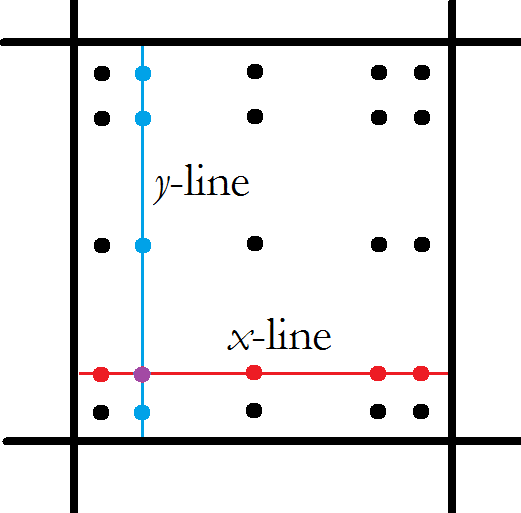
\includegraphics[width=3.5in]{lineDGelemDiag.PNG}
\caption{\label{fig:DGtensorSplit}The splitting of nodal contributions along "line-wise" directions on a tensor grid.}
\end{figure}

\be \frac{\partial \omega_{ij}}{\partial t} = (\frac{\partial \omega_{ij}}{\partial t})_{x-line} + (\frac{\partial \omega_{ij}}{\partial t})_{y-line} \ee

%
\section{Flux Interpolation}
The flux interpolant can be thought of  as either the interpolation of the product of the velocity and vorticity, or the product of the interpolations of velocity and vorticity; the result of these two interpolants are identical at the nodes
\be I_N f(x_i) = I_N(u(x_i) \omega(x_i)) = I_N(u(x_i)) I_N(\omega(x_i)) \ee
Furthermore, if we perform a Gauss-Legendre quadrature with collocated nodes, the quadrature is exact and the integral of either choice is equal
\be \int f \;dx \approx \sum_i^M u_i \omega_i w_i = \sum_i^M u_i \sum_j^M \omega_j \int \ell_i \ell_j \ee
The interpolation of the product may be order $M$, while the product of the interpolations is order $2M$, but the integral of either is equal; deciding between the two options may appear to be inconsequential. Consider however the case where we wish to integrate the product of the interpolated flux and the derivative of the weighting function. The interpolation of the product is order M and the derivative of the weighting basis M-1, the collocated Gauss-Legendre quadrature is exact

\be \int I_N(f) \, \ell_j'(x) \;dx = \sum_i^M u_i\omega_i \ell_j'(x_i) \ee

There is an important decision that has been implicitly made however. By choosing the quadrature of this form we are choosing the interpolant of the product. The two different flux interpolation choices no longer result in the same integral value. Importantly this means if we expect to need the full interpolatory order N of both the velocity and the vorticity in the stiffness integral, we will not be able to recover them. Instead we will recover the Nth order interpolant of them.

To retain the full order of each quantity, as well as suffer no quadrature error, we would have to instead evaluate the integral of the form
\be \begin{split}\int u(x) \omega(x) \ell_j'(x) \;dx &\approx \int \sum_i^M u_i \ell_i(x) \sum_k^M \omega_k \ell_k(x) \;\ell_j'(x) \;dx\\
&=\sum_i^M u_i \sum_k^M \omega_k \int \ell_i(x) \ell_k(x) \ell_j'(x) \;dx
\end{split}\ee
We will do this in the next section.
%
\section{Modified Quadrature}
To retain full interpolatory order of both the velocity and vorticity in the stiffness integral we seek a set of quadrature weights derived from
\be \sum_i^M u_i \sum_k^M \omega_k \;w_{unknown} = \sum_i^M u_i \sum_k^M \omega_k \int \ell_i(x) \ell_k(x) \ell_j'(x) \;dx \ee
note that we might alternatively wish to find something that looks more like the Gauss-Legendre quadrature rule
\be \sum_i^M u_i \sum_k^M \omega_k \sum_q^M \ell_j'(x_q) \;w_{unknown2} \ee
However we can actually go about it better keeping the derivative weighting basis inside the integral.
The derivative of the weighting basis can be derived analytically by use of logarithmic differentiation
\be f' = f \, [ln(f)]' \rightarrow \ell_j'(x)=\ell_j(x) \sum_{\substack{p=0\\ p\neq j}}^M \frac{1}{(x-x_p)} \ee
the resultant form can now be included in the integral.

The integral of the Lagrange basis functions associated with each interpolation times the derivative of the weighting basis must equal the quadrature weight associated that particular integrand, that is rather than M+1  quadrature weights associated with the M+1 nodes of the interpolation of the product, we have the associated $N(M+1)^2$ weights (where N is the number of possible weighting bases, for Galerkin methods N=M of course)
\be \int \ell_i(x) \ell_k(x) \ell_j'(x) \;dx = \mathbf{W}_{ikj} \ee
The integral can be done numerically by means of a normal Gauss quadrature of order at least $3M-1$ to be exact. These weights are pre-calculated at the start of the solver and saved for re-use.

The resultant modified quadrature now takes the form
\ben{modQuad} \int u(x) \omega(x) \ell_j'(x) \;dx \approx \mathbf{u}_i^T \mathbf{W}_{ikj} \, \boldsymbol{\omega}_k \ee
for each $j$th weighting basis function.

This may seem to incur a high cost, until one considers several facts:
\begin{itemize}
\item Normal Gauss-Legendre quadrature requires the stiffness integral be calculated for each weighting basis already, so the $j$ dimension of the quadrature matrix is no worse than before. 
\item One is able to extract \textit{more} information out of the \textit{same} number of interpolation points and achieve superior convergence of the stiffness integral than the standard Gauss-Legendre rule. B
\item By including the derivative of the weighting basis in the integral for the quadrature weight matrix, we integrate it exactly a priori. It never appears in the later quadrature of the stiffness integral except implicitly in the quadrature weight matrix itself.
\item The order and definition of the Lagrange basis functions for the vorticity and velocity interpolations are \textit{decoupled}. It is not necessary for the order of the velocity interpolation to be equal to the vorticity. Indeed, the set of interpolation nodes don't even have to be of the same \textit{kind}. It is completely permissible for example to have the vorticity nodes be the Gauss-Legendre nodes, and the velocity nodes to be Lobatto nodes.
\end{itemize}

This has significant advantages for the overall method, both in terms of minimizing both interpolation and quadrature error, as well as giving excellent flexibility in the solver. Normally to vary the order of the velocity interpolation one would need to re-interpolate at the vorticity nodes to recover the flux interpolant. This adds additional interpolation error, as well as potential aliasing problems. This additional interpolation step would also require about the same number of operations as using the larger quadrature weight matrix, making the two about equal in terms of computational cost. Instead one is free to choose the velocity order freely and the solver adapts seamlessly.

There is an additional computational savings as well. Although we would prefer to use the Legendre points for the vorticity (to preserve the diagonal mass matrix structure that we shall discuss in a coming section), we would like to use Lobatto points for the velocity. Ordinarily we would have to evaluate the boundary velocities and then leave them unused in the stiffness integral with normal Gauss-Legendre quadrature; both the vorticity and velocity would have to share the same  nodes or face re-interpolation costs. This adds wasted velocity evaluations which are the most expensive operation. One might be tempted to only evaluate the velocity at the Legendre points and extrapolate the velocity at the boundaries, but there is no guarantee that the two interpolated velocities from adjacent elements would agree; this would present obvious challenges in the boundary flux evaluation. However by using the modified quadrature matrix one can freely mix node sets, meaning the boundary velocity values are reused in the stiffness integral.

The maximum order polynomial that can be integrated exactly is also similar to some composite quadrature rules (such as Gauss-Kronrod \cite{Roni}): the order depends on whether the number of nodes is odd or even. An even node basis for one of the bases results in a $2M+1$ order accurate method, odd node number results in a $2M$ order accurate method (still sufficient to exactly integrate the product of two Mth order interpolants). A script in \S \ref{Algs} validates the convergence claims and order of accuracy of the modified quadrature method.

Table \ref{table:QuadMod} reports an example convergence study for a mixed order/type run with an 7th order Gauss-Legendre and 9th order Gauss-Lobatto quadrature rule showing quadrature error to within machine precision up to order $M+N+1$. It also compares the error in the interpolation of product (IoP) and product of interpolants (PoI), with the latter being an order of magnitude more accurate for this set of example functions.

\begin{table}
\centering
\caption{Convergence of Modified Quadrature for a 7/9th order Method}\label{table:QuadMod}
\begin{tabular}{llllll}
\hline
Order M+N & IoP       & PoI      & Quad. Error & Discretiz. Error &  Order M  \\ \hline
5         & -0.0543   & 0.234    & 2.22e-16         & 0.234                & 3  \\
7         & 0.0162    & 0.0182   & -5.55e-16        & 0.0182               & 4  \\
9         & -0.0143   & 0.0493   & -1.67e-16        & 0.0493               & 5  \\
11        & 0.00342   & 0.00133  & 2.22e-16         & 0.00133              & 6  \\
13        & -0.00182  & 0.00375  & 5.00e-16         & 0.00375              & 7  \\
15        & 0.000445  & 9.38e-05 & 5.55e-16         & 9.38e-05             & 8  \\
17        & -0.000161 & 0.000139 & 8.33e-16         & 0.000139             & 9  \\
19        & 4.20e-05  & 6.15e-06 & 0.000326         & 0.000332             & 10 \\
21        & -1.11e-05 & 2.90e-06 & 0.000523         & 0.000526             & 11 \\
23        & 3.15e-06  & 3.37e-07 & -9.75e-05        & -9.72e-05            & 12 \\ \hline
\end{tabular}
\end{table}

%------------------------------------
\chapter{Implementation}
\section{Overall Solver Structure}
It is worth briefly mentioning the overall structure of the solver, as it motivates some of the machinery developed and provides a useful overview of the detailed portions of the following sections. The preamble contains various solver configuration parameters and initializes most of the persistent data objects. It also initializes quadrature information which in turn is used to initialize the quadrature weight matrices needed for the order of the vorticity and velocity. The quadrature matrix is modified in place to incorporate the Jacobian as well as the inverse Mass matrix entry so that these do not needed to be multiplied by after the fact.

Most data is stored in one of two different formats, either a column-major form that matches Matlab's memory layout to optimize indexing performance, or a "line-wise" format. The line-wise terminology shouldn't be confused with any physical phenomenon, rather it relates to the tensor composition of the code. As the $x$ and $y$ direction problems are largely decoupled, each is treated independently, with a "line" being a particular 1D basis along the coordinate direction. Adjacent lines are parallel 1D basis functions that share a boundary node. For an example layout of $x$ and $y$ lines see Figure~\ref{fig:streams}.
\begin{figure}
\centering
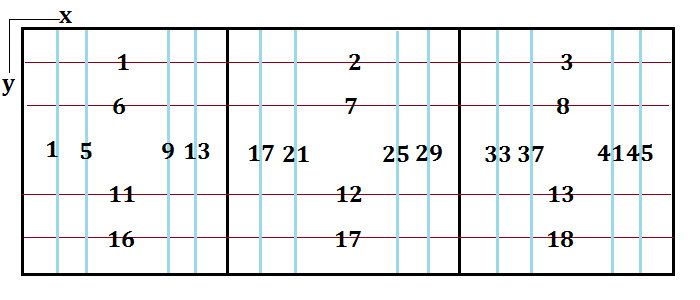
\includegraphics[width=5.5in]{streams.PNG}
\caption{\label{fig:streams}"Line-wise" numbering for elements 1, 5, and 9 in a 4x5 element global domain.}
\end{figure}
The next section of the solver creates element-line-boundary-node associativity. These are used to freely select the appropriate sections of data associated with a particular hierarchy. Most of these are simply a column-wise index list, some are specifically shaped so that the returned data from the index selection is the correct shape for reuse (ND matrix etc). This is also where the coordinates of the vorticity nodes, velocity boundary nodes, and velocity internal element nodes are specified. 

The next section consists of a cell list of functions that specify the initial conditions of the system. The resultant initial condition is the linear superposition of all the selected generating functions. The interpolation vectors for the surface flux are constructed, again incorporating the Jacobian and inverse matrix entry like in the quadrature weight matrix to avoid element-wise multiplications later. Finally the "global" kernel evaluation matrices are constructed for later re-use (these will be described in greater detail in a following section).

At this point the remainder of the code occurs inside the main time marching loop. An explicit Runge-Kutta routine is used with an inner loop used for stage-stepping. Depending on the solver setup, the velocity evaluation code is either executed every time step, or every stage. The sum of the vorticity in each element is computed and those above a threshold are added to element-wise and line-wise masks. Each element in the mask is treated as a source of vorticity and the velocity from that element is added to the current running total for the global velocity. Total element and element boundary velocities are formed for later use in the semi-discrete system.

The DG advection code always occurs within the RK stage loop. Vorticity is extrapolated at the element boundary. Boundary conditions are applied and the element boundary fluxes are evaluated. The stiffness term is evaluated for the current stage's vorticity and velocity configuration. At this point the semi-discrete system is complete and the stage's rate of change for all nodes is computed for each direction and the two are added together. The new vorticity is computed for the stage and both the time-stepping and stage-stepping loops wrap.

There is also some additional post-processing type routines that run that save simulation data for later use, and can also update in realtime displaying current simulation health statistics ($L^2$ norm etc.).
%
\section{Mass Matrix}
As discussed in the Interpolation Node Choice section, the set of Legendre roots for the vorticity interpolation points results in
\be \int \ell_i(x) \ell_j(x) dx = \delta_{ij} w_j \ee
This proves particular useful for the mass term, meaning the choice of Legendre nodes for interpolation results in a diagonal mass matrix that is trivially invertible. \eqref{DGJoshTemp} is then simplified to
\ben{DGJoshTemp2} \frac{d \aomega_j}{dt} \frac{w_j \Delta x}{2}
+\hat{f}\ell_j \Big|^{x_R}_{x_L} 
- \int_{-1}^{1} f(\aomega) \, \ell_j' \;dX = 0 \ee

One could instead choose the set of Lobatto points to avoid extrapolating the vorticity at the element boundaries, but this would result in a full mass matrix that when inverted necessitates a matrix-vector product which is about as computationally expensive as extrapolating the boundary vorticity.
%
\section{Usefulness of Structured Tensor Mesh}
The test cases that are considered in this thesis are all free of impinging geometry and have no bias known a priori, as such a constant-size structured mesh comprised of squares is used. It is worth noting that this is by no means required, an un-structured mesh is easily treated via a mapping to a canonical computational element \cite{Persson2013}. The structured mesh merely affords ease of implementation, as well as simplification of element-line-boundary-node indexing.

Likewise, the tensor product basis used for the vorticity can be exploited for computational and ease-of-implementation gains. The tensor product means that the 2D integral of the vorticity times the Biot-Savart kernel can be reduced by a matrix-vector and vector-vector product by pre-multiplying the vorticity of a source by the outer product of the Gauss-Legendre weights component-wise, which is then reused for each kernel-vorticity integration.
\be \int \omega \times K \;dx \approx \boldsymbol{w}^T(\boldsymbol{\omega}_E.*\boldsymbol{K}) \boldsymbol{w} \rightarrow (\boldsymbol{ww}^T.*\boldsymbol{\omega})\boldsymbol{K} \ee
where ".*" indicates element-wise multiplication per Matlab convention. It's worth noting that the pre-multiplied product and the kernel are reshaped to be row and column vectors respectively. If there are many kernels to be integrated for a particular vorticity source the computational savings are appreciable.
%
\section{Stiffness Matrix}
We can apply the results for the modified quadrature rule from \eqref{modQuad} to the purpose of evaluating the stiffness integral we have left unevaluated thus far. Recall that for maximum flexibility the velocity interpolation order is independent of the vorticity order. In addition the Lobatto points are chosen for the velocity to reuse the boundary velocities. At first glance it might seem actually counter productive to choose a different order or set of nodes for the velocity. To avoid needing "off-line" interpolation the velocity nodes should be co-linear with the vorticity lines. The result for a 5th order velocity and vorticity field is shown in Figure~\ref{fig:VelocityLobatto}.

It would appear we actually need double the velocity evaluation points! How could this be a savings over collocated velocity points? The non-square tensor product of the Lobatto nodes with the Legendre nodes means that the $x$-line velocity nodes will never coincide with the $y$-line velocity nodes.

The answer is that the velocity is evaluated component-wise. Along the $x$-line we only require $u_x$ and along the $y$-line we only require $u_y$. We do not need need the other velocity component at any particular velocity node, so though they may not coincide we don not miss out on any opportunities. The trade-off is that the velocity field is perhaps a bit harder to post-process, but if the result cuts in half the expected runtime of the most expensive portion of the method it seems a fair trade-off.

We can now happily apply the modified quadrature matrix to our elemental PDE
\ben{DGJoshTemp3} \frac{d \aomega_j}{dt} \frac{w_j \Delta x}{2}
+\hat{f}\ell_j \Big|^{x_R}_{x_L} 
- \mathbf{u}^T \mathbf{W}_{--j} \, \boldsymbol{\omega} = 0 \ee
rearranging to obtain the rate of change of the nodal vorticity
\ben{DGJosh} \frac{d \aomega_j}{dt}
=\frac{2}{w_j \Delta x} \left[\mathbf{u}^T \mathbf{W}_{--j} \, \boldsymbol{\omega} - \hat{f}\ell_j \Big|^{x_R}_{x_L}\right]  \ee
This nodal equation now describes the line's contribution to the time evolution of a particular node. This calculation is performed for all vorticity nodes on all $x$-lines and added to the rate of change of the matching vorticity nodes in the $y$-lines.

\begin{figure}
\centering
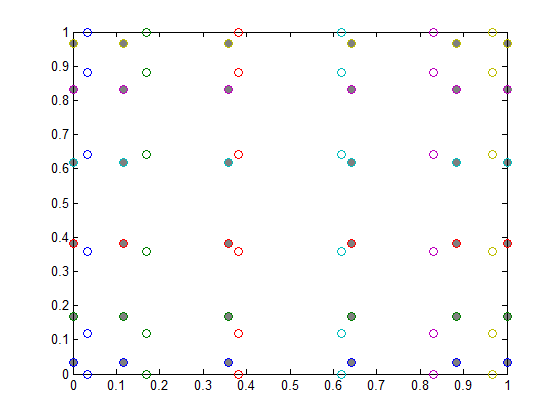
\includegraphics[width=5.5in]{VelocityLobatto.PNG}
\caption{\label{fig:VelocityLobatto}5$^{th}$ order Lobatto velocity nodes along $x$-lines (dark circles) and $y$-lines (empty circles).}
\end{figure}

%
\section{Vortex Sparseness}
One of the advantages of DG as an advection scheme is the compact local support of the vorticity. This means that for a large domain with only sparse vorticity one should be able to only consider those elements that contain vorticity. The sparseness can be applied in several ways. From the DG perspective, if an element is empty than there is nothing to advect and the element can be left out of evaluation entirely. The reality is that even small numerical errors in the boundary flux may lead to non-physical perturbations in the vorticity field in what should be otherwise empty elements. These elements can now now not be ignored, lest some instability result from not properly handling non-zero elements.

The reality is of course from a vorticity-velocity perspective these elements are unimportant, even if they are important from a consistency standpoint for the DG part of the code. Therefore a threshold value can be specified, elements with total vorticity less that the threshold value are ignored, and only those elements above the threshold are put in a mask. The masked elements are the ones considered as sources for the velocity evaluation. Additionally, only the boundary velocities for these unimportant elements are calculated and a reduced velocity order stiffness term is calculated for them.

The current state of the solver is bottlenecked by the velocity evaluation, so although some savings would be realized by maintaining true vorticity domain sparseness, the result is that it has little impact on the overall speed of the solver. The unmasked elements have only a marginal impact on the cost of the velocity evaluations. However empty elements do have one major effect on solver performance, this will be discussed in the next section.

%
\section{Velocity Evaluation}
For ease of implementation and to eliminate the effects of as most approximation error as possible on validation, the velocity is evaluated directly at each Lobatto velocity (only the boundary nodes for the unmasked elements) by means of the Biot-Savart integral. It is important to note that has $\mathcal{O}(N^2)$ complexity, and so the runtime rapidly reaches a limit of impracticality above a limit.

The velocity at a particular node is calculated by summing the net effect of each masked source element. A loop steps through each source element and adds it's contribution to all velocity nodes. The actual source-node pair evaluation is done via a regular Gauss-Legendre quadrature of order equal to the vorticity field. For the far field this performs as expected, with excellent convergence. However for elements directly neighboring the source element, as well as the source element itself, the nearly singular nature of the integral poses convergence problems for the quadrature.

This is unsurprising; the weighting function for the Legendre polynomials is simply $w_{Leg}(x)=1$. As such, the product of the kernel and the vorticity near the source element is poorly interpolated by a polynomial. Ideally one would use a weighting function of a form similar to the singular portion of the kernel to form a new orthogonal basis, but here one is limited by the tensor basis. More freedom is required in the interpolation points to provide adequate leeway to generate desirable quadrature rules. The generation of general multivariable interpolation and quadrature bases is an area of active and relatively recent effort \cite{Gasca2000,Xu2012,Gautschi2013}.

At first one might think that the predominant bottleneck in the scaling of the velocity evaluation is simply the evaluation of the Biot-Savart integral. While this may be the case in other codes, or other workstation setups, this actually only accounts for typically less than half the cost. The majority of the cost actually results from the assembly of the kernel values. One is presented with three options: calculate a new set of kernel values for each source element, form a "global" matrix of kernel values that one maps to the particular source element under consideration, or directly calculating and storing kernel values for every source-node pair.

The first choice is the most direct, but also the slowest. It is bottlenecked by computational cost; the number of operations to form the kernel actually exceeds those needed to evaluate the integral. The third method is the fastest, but bound by memory constraints which scale as $Np^4 K^4$. Even a modest 5th order velocity method with 20x20 elements (~15k DOF) would require 1.8Gb of memory to store.

The second method is the one currently used in the code. The global domain is reflected about both axes for a central element and the kernel values are calculated for all elements in relation to the reference source. Depending on where the actual source element is in the true domain determines what portion of the "global" domain is selected with respect to the reference element, see Figure~\ref{fig:GlobalKernel}. This realizes significant computational savings from not having to repeatedly recalculate the kernel values, however it is memory access bottlenecked. Repeatedly selecting and manipulating non-contiguous blocks of memory can be slow. Even being careful to arrange as much data column-major as possible only delays the problem.

This also means otherwise "empty" elements affect performance by further fragmenting the global kernel matrix. At some point the sparseness of the domain is sufficient that the recalculation of the kernel for each source outperforms an overly fragmented global matrix. A hybrid method that uses as much memory as reasonable to store kernel values for the elements with the greatest vorticity, and calculates all others on-the-fly would be the most efficient use of resources and was considered but development time did not permit it's construction. Note that the memory bottleneck limitation is not an intrinsic property of the underlying method itself, but rather a consequence of the solver implementation and Matlab's underlying memory model.

\begin{figure}
\centering
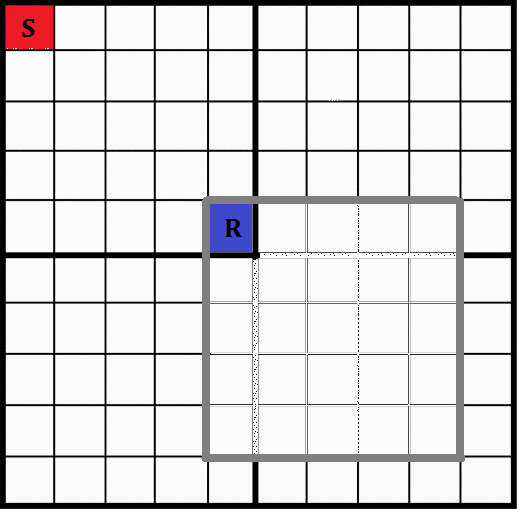
\includegraphics[width=5.5in]{GlobalKernel.PNG}
\caption{\label{fig:GlobalKernel}The "global" kernel matrix showing (R)eference source and actual (S)ource, the upper left quadrant is the actual full domain, the selected region with respect to (R) selects the correct values of the kernel for (S).}
\end{figure}

%
\section{Reduced Order Velocity (Global/Far-field)}
The flexibility permitted by the modified quadrature matrix allows a choice of velocity order independent of the vorticity order. A reduced velocity order reduces the runtime of the solver significantly, but this comes with some potentially severe drawbacks as will be shown. The reduced order velocity field is most easily applied to unmasked elements, but can also be extended to far-field elements. The stiffness integral can be broken up into low and high order pieces with self, neighboring, and nearby elements evaluated at high order, and slowly changing far-field elements at reduced velocity order.

In some senses a reduced order far-field component is an analogue to the cluster-cluster interactions of a fast multipole method. The implementation of the reduced order far-field evaluations is deferred to a later extension of the code that will fully implement a FMM-like evaluation.
%
\section{Explicit Time-Stepping}
With the semi-discrete system formed, one must now choose how to discretize in time. For simplicity an explicit time-stepping method will be used. The two chief categories are multi-step and multi-stage methods, typically either Adams-Bashforth or Runge-Kutta respectively. It is known that Forward Euler and AB2 are unstable for DG with an upwind flux due to it's dissipative nature. The choices permitted then are Runge-Kutta or a higher-order Adams-Bashforth.

The recent thesis work of Atcheson \cite{Reid} presents an excellent overview of the optimal choice of time-stepping algorithm for a DG operator. In particular it was shown that Runge-Kutta methods outperformed AB3 and that all higher-order Adams-Bashforth schemes required far too restrictive of a time-step to satisfy the CFL condition to be efficient. Out of all the Runge-Kutta schemes considered \cite{Toulorge} one of the competitive options was the "NRK14C" scheme developed by Niegemann et al. \cite{Niegemann}. This is an optimized 4th order, 14 stage low storage scheme of similar structure to other 2N style schemes \cite{Carpenter}.

Notably, NRK14C permits a time-step 1.86 times as long per stage than the canonical RK4 assuming the limitation is the negative real component in the stability region of the method. This equates to a proportional runtime decrease for almost negligible implementation effort. 

There is one further choice to be made regarding time-stepping: where to include the velocity evaluation. It is reasonable to assume that in practice the numerical stiffness of the problem is due to the DG operator, not the velocity evaluation. This means one is free to either evaluate the velocity at each stage, or instead to evaluate at the start of each step. 

Of course the time discretization error of the velocity field will be increased, but the runtime of the resultant method will be an order of magnitude faster. If the CFL condition is stringent enough to necessitate a small time-step compared to the evolution rate of the velocity, the velocity evaluation is moved outside of the stage loop. The effect on the overall convergence of the method is important to consider when making this choice.

%
\section{Validation and Convergence of Proposed Methods}
\subsection{Perlmann: Stationary Vortex}
Of primary interest in the development of a new method is validation of it with common test cases, as well as an evaluation of convergence. Perlmann's 7th order polynomial was the first case studied \cite{Perlmann1985}. The intial condition is a stationary vortex that permits an analytical solution to compare against. The initial vorticity distribution is of the form
\be \omega(z)=(1-|z|^2)^7, \; |z|\leq 1  \quad \omega(z)=0, \;|z|>1 \quad z^2=x^2+y^2 \ee
The $L^2$ norm and total vorticity in the domain are plotted to determine if the resultant advected vorticity matches the expected analytical result.

\subsection{Strain: Interacting Vortex Patches}
Strain's system of interacting random vortex patches \cite{Strain1996} forms the next validation case. Specific initial conditions are specified for each of the vortex patches in Table \ref{table:StrainTable} with the overall system consisting of the linear superposition of each patch
\be \omega(x,y,0) = \sum_{j=1}^m \Omega_j exp(-((x-x_j)^2 + (y-y_j)^2)/\rho_j^2) \ee
An explicit data set for the results is not reported, but a set of contour plots illustrates the time evolution. The same parameters are used in the present solver and similar contour plots are compared against the validating set.

\begin{table}
\centering
\caption{Interacting Vortex Patch Parameters}\label{table:StrainTable}
\begin{tabular}{lllll}
\hline
j & $x_j$    & $y_j$    & $\rho_j$ & $\Omega_j$ \\ \hline
1 & -0.6988 & -1.7756 & 0.6768  & -0.4515   \\
2 & 1.4363  & -1.4566 & 0.3294  & 0.4968    \\
3 & -0.1722 & 0.4175  & 0.5807  & -0.9643   \\
4 & -1.5009 & -0.0937 & 0.2504  &  0.3418    \\ \hline
\end{tabular}
\end{table}

\subsection{Koumoutsakos: Elliptical Vortex}
The final validation case is the evolution of an elliptical vortex patch \cite{Koum1997}. The specific initial configuration is specified as
\be \omega^{II}(r) = 20(1-(r/0.8)^4), \; r\leq 0.8 \quad \omega^{II}(r)=0, \; r>0.8 \ee
however the cases tested were actually elliptical, to accommodate this the initial distribution was modified to
\be \omega^{II}(x,y,0)_{mod} = 20(1-((x/a)^2+(y/b)^2)^2/0.8^4 ) \quad a=1, \; b=2 \ee
The contour levels are specified in the resultant figure as 0.25, 0.50, 1, 2, ..., 20; these levels are used in the current code's resultant plot for direct comparison.

\subsection{Other}
Analytical convergence rate of the method at various order vorticity fields, velocity fields, velocity evaluation step/stage-wise, effective core sizes, and long time integrations also take advantage of the analytical solution available from the Perlmann test case. The elliptical patch and system of interacting  patches also receive a qualitative assessment of the convergence rate, and their dependence on the test parameters.

%------------------------------------
\chapter{Results}
\section{Validation}
\subsection{Perlmann: Stationary Vortex}
Although it is expected that in the stationary vortex case the choice of stage or step-wise velocity evaluation shouldn't matter, to minimize any sources of error or confounding factors a stage-wise evaluation was used during validation studies. To fully validate the method the largest combination of order and number of elements was chosen that still permitted a reasonable runtime to 48 seconds. This is close to 4 full revolutions, where the period is $T_p = \frac{4 \pi}{\omega_{max}}$. This test is denoted P1 and the test conditions (along with all other test cases) are tabulated in \ref{table:TestVars}. All plots likewise are marked with the test case number.

To examine the long-term behavior of the method the $L^2$ norm of the error \ref{fig:L2P1} as well as the dissipation of the total vorticity in the domain \ref{fig:wtotP1} are plotted through the course of the vortex evolution. The final surface plot and contour plot can be seen in Figures \ref{fig:P1surf} and \ref{fig:P1cont} respectively.

\subsection{Strain: Interacting Vortex Patches}

\subsection{Koumoutsakos: Elliptical Vortex}

\section{Convergence}
\subsection{Perlmann: Stationary Vortex}

\subsection{Strain: Interacting Vortex Patches}

\subsection{Koumoutsakos: Elliptical Vortex}


\section{Stage vs. Step-wise Velocity Evaluation}

\section{Reduced Order Velocity}

\section{Runtime Speed and Memory Footprint of Solver}
%------------------------------------
\chapter{Discussion}
\section{Analytical Validation of Model}
Comparison of existing analytical solutions vs model (Euler vortex, 5th order poly, other Saffmann test cases)
\newpage.
\newpage
\section{Empirical Convergence of Method}
\newpage.
\newpage
\section{Computational Efficiency}
\newpage.
\newpage
\section{Extended Body Fast Multipole Formulation}
%------------------------------------
\chapter{Conclusion}
%------------------------------------
\chapter{Recommendations}
\section{Extension to 3D}
\section{Flux Limiters}
\section{Impinging Geometry and Boundary Conditions}
\section{Viscosity}
\newpage
\section{Implicit and Local Time Stepping}
\section{Parallelizability}
\section{FMM Improvements}
\section{2D Non-classical Quadrature for Nearly Singular Integrands}
%------------------------------------
\chapter{Notable Code and Algorithms}\label{Algs}
\section{Modified Two-part quadrature}

It is applied to the integration of the product of $M$ and $N=M-1$ order functions, with M varying over a particular range. The interpolation of the product (IoP) and product of the interpolants (PoI) were numerically integrated by Matlab's built-in adaptive quadrature routine until machine precision was 

Vectorized Lagrange evaluation, Lagrange derivatives, etc
\newpage
\section{Binary Singleton Expansion Matrix-Vector Products}
\section{Lagrange Bases and Constructed Quadrature}
\newpage
\section{Velocity Evaluation}
\section{Semi-discrete System Construction}
\newpage
\section{Low-storage Stability Optimized Runge-Kutta}
%------------------------------------
\chapter{Literature Cited}
\begin{thebibliography}{9}
%Overview
\bibitem{Lugt1983}
H. J. Lugt, Vortex Flow in Nature and Technology, Krieger Publishing Company, Malabar, FL, USA, 1983.
\bibitem{Saffman1992}
P. G. Saffman, Vortex Dynamics, Cambridge Univ. Press, Cambridge, UK, 1992.
\bibitem{Speziale1987}
C. G. Speziale, On the advantages of the vorticity-velocity formulation of the equations of fluid dynamics, J. Comput. Phys. 73 (1987) 476-480.
%Point methods
\bibitem{Point1}
L. Rosenhead, The formation of vorticies from a surface of discontinuity, Proc. Roy. Soc. London Ser. A 134 (1931) 170-192.
\bibitem{Point2}
G. Birkhoff, J. Fisher, Do vortex sheets roll up?, Rend. Circ. Math. Palermo, Ser. 2 8 (1959) 77-90.
\bibitem{Point3}
F. H. Abernathy, R. E. Kronauer, The formation of vortex streets, J.Fluid Mech. 13 (1962) 1-20.
\bibitem{Point4}
A. J. Chorin, P. S. Bernard, Discretization of a vortex sheet, with an example of roll-up, J. Comput. Phys. 13 (3) (1973) 423-429.
\bibitem{Point5}
K. Kuwahara, H. Takami, Numerical studies of two-dimensional vortex motion by a system of point vortices, J. Physical Society of Japan 34 (1) (1973) 247-253.
\bibitem{Point6}
R. G. Zalosh, Discretized simulation of vortex sheet evolution with buoyancy and surface tension effects, AIAA Journal 14 (11) (1976) 1517-1523.
%Line methods
\bibitem{Line1}
G. K. Batchelor, An Introduction to Fluid Dynamics, Cambridge University Press, 1967, 1973.
\bibitem{Line2}
W. T. Ashurst, E. Meiburg, Three-dimensional shear layers via vortex dynamics, J. Fluid Mech. 189 (1988) 87-116.
\bibitem{Line3}
J. E. Martin, E. Meiburg, Numerical investigation of three-dimensional evolving jets subject to axisymmetric and azimuthal perturbation, J. Fluid Mech. 230 (1991) 271-318.
\bibitem{Line4}
A. Leonard, Numerical simulation of interacting, three-dimensional vortex filaments, in: Proceedings of the IV Intl. Conference on Numerical Methods of Fluid Dynamics, no. 35 in Lecture Notes in Physics, Springer-Verlag, 1975, pp. 245-250.
%Sheet methods
\bibitem{Sheet1}
M. E. Agishtein, A. A. Migdal, Dynamics of vortex surfaces in three dimensions: Theory and simulations, Physica D 40 (1989) 91-118.
\bibitem{Sheet2}
O. M. Knio, A. F. Ghoniem, Three-dimensional vortex simulation of rollup and entrainment in a shear layer, J. Comput. Phys. 97 (1991) 172-223.
\bibitem{Sheet3}
O. M. Knio, A. F. Ghoniem, Vortex simulation of a three-dimensional reacting shear layer with in finite-rate kinetics, AIAA J. 30 (1) (1992) 105-116.
%Volume methods
\bibitem{Volumes1}
G. Russo, J. A. Strain, Fast triangulated vortex methods for the 2D Euler equations, J. Comput. Phys. 111 (1994) 291-323.
\bibitem{Volumes2}
M. Carley, A triangulated vortex method for the axisymmetric Euler equations, J. Comput. Phys. 180 (2002) 616-641.
\bibitem{Volumes3}
S. A. Huyer, J. R. Grant, Solution of two-dimensional vorticity equation on a Lagrangian mesh, AIAA Journal 38 (5) (2000) 774-783.
%Remeshing problems
\bibitem{Remesh2}
J. T. Beale, On the accuracy of vortex methods at large times, in: IMA Workshop on Computational Fluid Dynamics and Reacting Gas Flows, Springer-Verlag, 1988, p. 19.
\bibitem{Remesh3}
J. S. Marshall, J. R. Grant, Penetration of a blade into a vortex core: vorticity response and unsteady blade forces, J. Fluid Mech. 306 (1996) 83-109.
\bibitem{Remesh4}
H. O. Nordmark, Rezoning for higher order vortex methods, J. Comput. Phys. 97 (1991) 366-397.
\bibitem{Remesh5}
H. N. Najm, R. B. Milne, K. D. Devine, S. N. Kempa, A coupled Lagrangian-Eulerian scheme for reacting flow modeling, ESAIM Proc. 7 (1999) 304-313.
%Convergence
\bibitem{Convg2D}
O. H. Hald, V. D. Prete, Convergence of vortex methods for Euler's equations, Math. Comput. 32 (1978) 791-809.
\bibitem{Convg3D}
J. T. Beale, A convergent 3-D vortex method with grid-free stretching, Math. Comput. 46 (174) (1986) 401-424.
%Brown
\bibitem{Brown2000}
 R.E. Brown. Rotor Wake Modeling for Flight Dynamic Simulation of Helicopters. AIAA Journal, 2000. Vol. 38(No. 1): p. 57-63.
\bibitem{Brown2004}
A.J. Line, R.E. Brown. Efficient High-Resolution Wake Modelling using the Vorticity Transport Equation. in 60th Annual Forum of the American Helicopter Society. 2004. Baltimore, MD.
%DG
\bibitem{ReedHill}
W.H Reed and T.R. Hill. Triangular mesh methods for the neutron transport equation. 1973.
\bibitem{Lesaint}
Lesaint, P., and Pierre-Arnaud Raviart. On a finite element method for solving the neutron transport equation. Mathematical aspects of finite elements in partial differential equations 33 (1974): 89-123.
\bibitem{Persson2013}
P.O. Persson. A Sparse and High-Order Accurate Line-Based Discontinuous Galerkin Method for Unstructured Meshes. J. Comp. Phys., Vol. 233, pp. 414-429, Jan 2013.
\bibitem{HestWar}
Hesthaven, Jan S., and Tim Warburton. Nodal discontinuous Galerkin methods: algorithms, analysis, and applications. Vol. 54. Springer Science \& Business Media, 2007.
%Important vortex papers
\bibitem{HaldReview}
Hald, Ole H. Convergence of vortex methods. Vortex methods and vortex motion. Vol. 1. 1991.
\bibitem{Hald3}
Hald, Ole H. Convergence of vortex methods for Euler's equations, III. SIAM journal on numerical analysis 24.3 (1987): 538-582.
\bibitem{WL}
Winckelmans, G. S., and A. Leonard. Contributions to vortex particle methods for the computation of three-dimensional incompressible unsteady flows. Journal of Computational Physics 109.2 (1993): 247-273.
\bibitem{BealeMajda}
Beale, J. Thomas, and Andrew Majda. High order accurate vortex methods with explicit velocity kernels. Journal of Computational Physics 58.2 (1985): 188-208.
\bibitem{Strain1997}
J. Strain. Fast adaptive 2D vortex methods. Journal of computational physics 132.1 (1997): 108-122.
\bibitem{LindsayKrasny2001}
K. Lindsay, and R. Krasny. A particle method and adaptive treecode for vortex sheet motion in three-dimensional flow. Journal of Computational Physics 172.2 (2001): 879-907.
\bibitem{Rosenhead1930}
L. Rosenhead. The spread of vorticity in the wake behind a cylinder, Proc. Roy. Soc. London Ser. A 127, 590 (1930).
\bibitem{Moore1972}
D. W. Moore. Finite amplitude waves on aircraft trailing vortices, Aero. Quart. 23, 307 (1972).
\bibitem{MoussaCarley2008}
Moussa, C., Carley, M. J. (2008). A Lagrangian vortex method for unbounded flows. International journal for numerical methods in fluids, 58(2), 161-181.
\bibitem{SteinhoffUnderhill1994}
J. Steinhoff, D. Underhill, Modification of the Euler equations for "vorticity confinement": Application to the computation of interacting vortex rings, Phys. Fluids 6 (8) (1994) 2738-2743.
%Test cases
\bibitem{Perlmann1985}
M. Perlman. On the accuracy of vortex methods, J. Comput. Phys. 59 (1985) 200–223.
\bibitem{Strain1996}
J. Strain. 2D vortex methods and singular quadrature rules. Journal of Computational Physics 124.1 (1996): 131-145.
\bibitem{Koum1997}
P. Koumoutsakos. Inviscid axisymmetrization of an elliptical vortex, J. Comput. Phys. 138 (1997) 821–857.
\bibitem{KoumLeonard1995}
Koumoutsakos, P., Leonard, A. (1995). High-resolution simulations of the flow around an impulsively started cylinder using vortex methods. Journal of Fluid Mechanics, 296, 1-38.
\bibitem{Southerland1991}
K. B. Southerland, J. R. P. III, W. J. A. Dahm, K. A. Buch. An experimental study of the molecular mixing process in an axisymmetric laminar vortex ring, Phys. Fluids A 3 (5) (1991) 1385–1392.
%Fast velocity eval
\bibitem{SchumannSweet1976}
Schumann, U., Sweet, R. A. (1976). A direct method for the solution of Poisson's equation with Neumann boundary conditions on a staggered grid of arbitrary size. Journal of Computational Physics, 20(2), 171-182.
\bibitem{BarnesHut1986}
Barnes, J.,  Hut, P. (1986). A hierarchical O (N log N) force-calculation algorithm.
\bibitem{GreengardRokhlin1987}
Greengard, L.,  Rokhlin, V. (1987). A fast algorithm for particle simulations. Journal of computational physics, 73(2), 325-348.
%General ortho bases
\bibitem{Gasca2000}
Gasca, Mariano, Thomas Sauer. Polynomial interpolation in several variables. Advances in Computational Mathematics 12.4 (2000): 377-410.
\bibitem{Xu2012}
Xu, Yuan. Minimal Cubature rules and polynomial interpolation in two variables. Journal of Approximation Theory 164.1 (2012): 6-30.
\bibitem{Gautschi2013}
Gautschi, Walter. Neutralizing nearby singularities in numerical quadrature. Numerical Algorithms 64.3 (2013): 417-425.
%LSERK
\bibitem{Reid}
Atcheson, Thomas. Explicit Discontinuous Galerkin Methods for Linear Hyperbolic Problems. Diss. Masters Thesis, Rice University. http://hdl. handle. net/1911/75120, 2013.
\bibitem{Toulorge}
Toulorge, Thomas, and Wim Desmet. Optimal Runge–Kutta schemes for discontinuous Galerkin space discretizations applied to wave propagation problems. Journal of Computational Physics 231.4 (2012): 2067-2091.
\bibitem{Niegemann}
Niegemann, Jens, Richard Diehl, and Kurt Busch. Efficient low-storage Runge–Kutta schemes with optimized stability regions. Journal of Computational Physics 231.2 (2012): 364-372.
\bibitem{Carpenter}
Carpenter, Mark H., and Christopher A. Kennedy. Fourth-order 2N-storage Runge-Kutta schemes. (1994).
%Misc
\bibitem{Roni}
Quarteroni, Alfio, and Alberto Valli. Numerical approximation of partial differential equations. Vol. 23. Springer Science \& Business Media, 2008.
\bibitem{Allen}
Allen, Myron B., and Eli L. Isaacson. Numerical analysis for applied science. Vol. 35. John Wiley \& sons, 2011.
\bibitem{Gustaf}
Gustafsson, Bertil. Fundamentals of Scientific Computing. Vol. 8. Springer Science \& Business Media, 2011.
%Licenses
\bibitem{KoumLic}
Reprinted from Publication title, Vol /edition number, Author(s), Title of article / title of chapter, Pages No., Copyright (Year), with permission from Elsevier [OR APPLICABLE SOCIETY COPYRIGHT OWNER]."
\bibitem{StrainLic}
Reprinted from Publication title, Vol /edition number, Author(s), Title of article / title of chapter, Pages No., Copyright (Year), with permission from Elsevier [OR APPLICABLE SOCIETY COPYRIGHT OWNER]."

%\bibitem{}
%\bibitem{}
%\bibitem{}
%\bibitem{}

\end{thebibliography}
%\begin{figure}
%\centering
%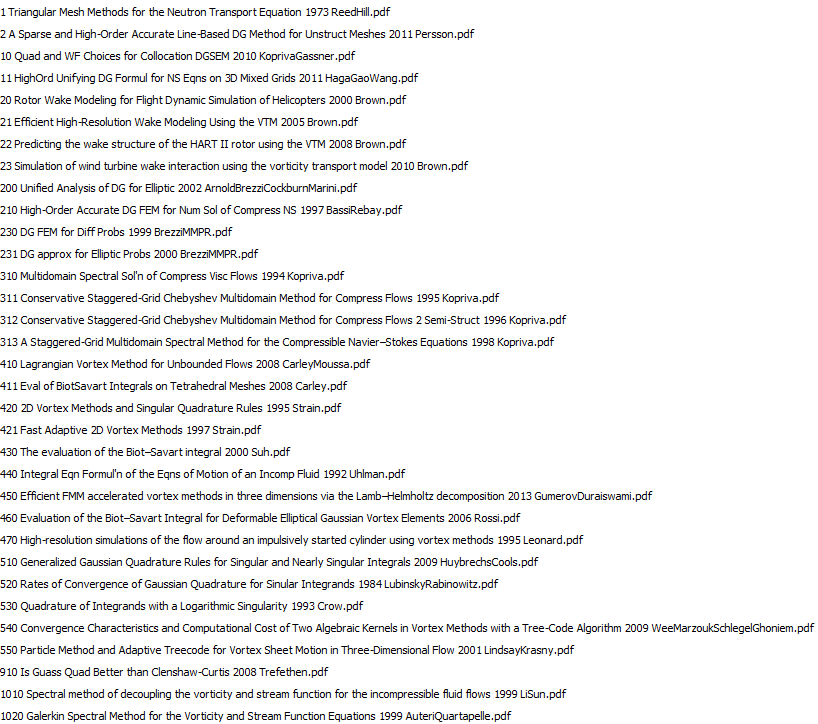
\includegraphics[width=1.4\textwidth]{LitStart.PNG}
%\caption{\label{fig:ring}Dirty preliminary lit cited.}
%\end{figure}

\end{document}